\documentclass[border=3pt]{standalone}
% Preâmbulo compartilhado pelos diagramas TikZ da aula 8 de Navegação (Implementação do RRT)
\usepackage[T1]{fontenc}
\usepackage[utf8]{inputenc}
\usepackage{lmodern}
\usepackage{amsmath}
\usepackage{xcolor}
\usepackage{tikz}
\usetikzlibrary{arrows.meta,angles,quotes,decorations.pathmorphing,decorations.pathreplacing,calc,
                positioning,shapes.geometric,shapes.misc,backgrounds,fit,
                math}

% Paleta (mesma dos SVGs originais)
\definecolor{dblue}{HTML}{2A5B8C}
\definecolor{dorange}{HTML}{B3541E}
\definecolor{dgreen}{HTML}{4A7C59}
\definecolor{dred}{HTML}{9C4B4B}
\definecolor{dcream}{HTML}{F4F1EA}
\definecolor{dshade}{HTML}{DDD7C9}

% Função gaussiana (não normalizada por padrão de escala visual)
\pgfmathdeclarefunction{gauss}{3}{%
  \pgfmathparse{1/(#3*sqrt(2*pi))*exp(-((#1-#2)^2)/(2*#3^2))}%
}

% Estilos comuns (prefixo d... para não colidir com chaves internas do pgf)
\tikzset{
  >={Stealth[length=2mm]},
  dguide/.style={gray!55, dashed, line width=0.4pt},
  daxis/.style={gray!60, line width=0.7pt, ->},
  dbody/.style={fill=black!3, draw=black!80, line width=1pt},
  dacc/.style={draw=dblue, line width=1pt},
  dlbl/.style={black!55, font=\small},
  dsub/.style={black!45, font=\footnotesize},
  dstate/.style={circle, draw=black!80, fill=dcream, line width=1pt,
                 minimum size=17mm, font=\large, inner sep=1pt},
  dobs/.style={circle, draw=black!80, fill=dshade, line width=1pt,
               minimum size=14mm, font=\large, inner sep=1pt},
  dbox/.style={rounded corners=2pt, draw=black!80, fill=dcream, line width=1pt,
               align=center, inner sep=6pt},
  dop/.style={circle, draw=black!80, fill=white, line width=1pt,
              minimum size=6mm, inner sep=0pt, font=\small},
  dtrans/.style={->, dblue, line width=1pt},
  dmeas/.style={->, dorange, line width=1pt},
  dcurve/.style={line width=1pt, dblue},
  dcurveb/.style={line width=1.4pt, dorange},
}

\begin{document}
\hyphenpenalty=10000 \exhyphenpenalty=10000 \tolerance=9999 \emergencystretch=3em
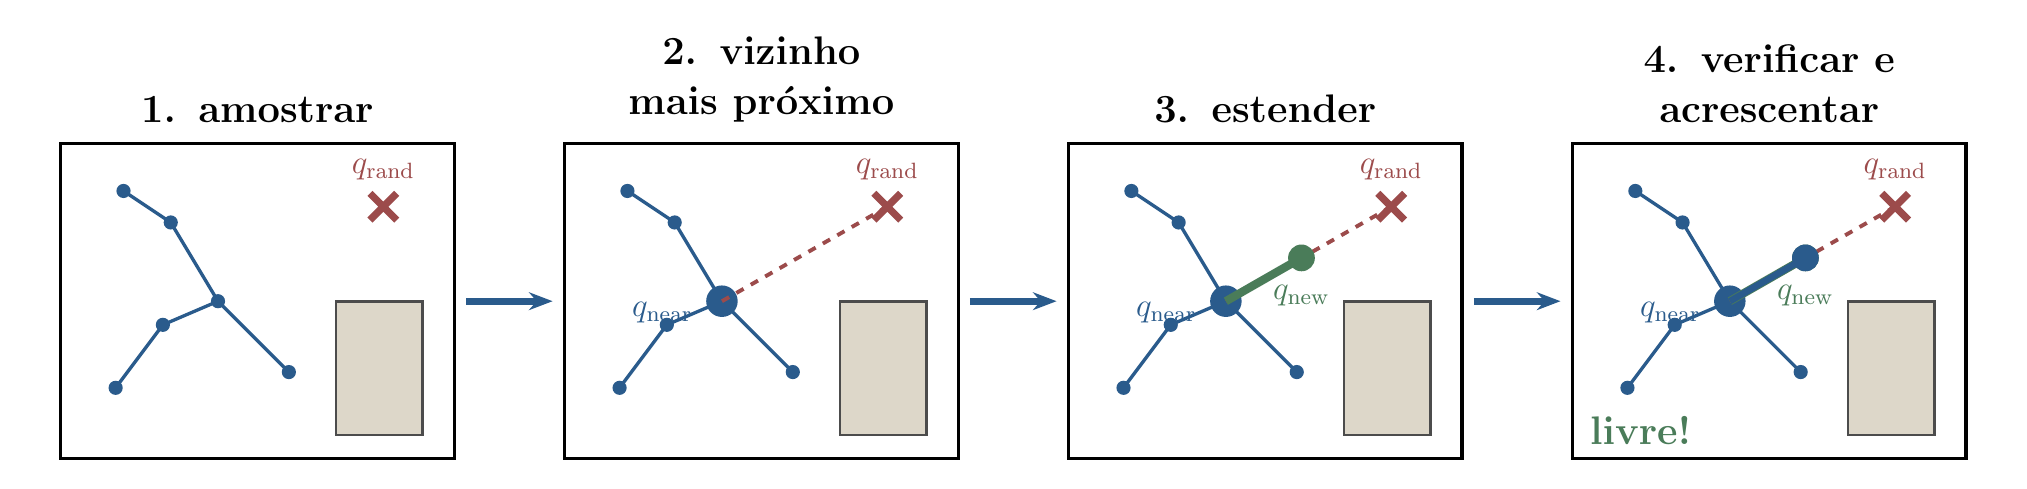
\begin{tikzpicture}[x=1cm,y=1cm]
\draw[line width=1.2pt, fill=white] (0.00,0) rectangle (5.00,4.00);
\draw[line width=1pt, draw=black!70, fill=dshade] (3.50,0.30) rectangle (4.60,2.00);
\draw[dblue, line width=1.2pt] (0.70,0.90) -- (1.30,1.70);
\draw[dblue, line width=1.2pt] (1.30,1.70) -- (2.00,2.00);
\draw[dblue, line width=1.2pt] (2.00,2.00) -- (1.40,3.00);
\draw[dblue, line width=1.2pt] (2.00,2.00) -- (2.90,1.10);
\draw[dblue, line width=1.2pt] (1.40,3.00) -- (0.80,3.40);
\fill[dblue] (0.70,0.90) circle (0.09);
\fill[dblue] (1.30,1.70) circle (0.09);
\fill[dblue] (2.00,2.00) circle (0.09);
\fill[dblue] (1.40,3.00) circle (0.09);
\fill[dblue] (2.90,1.10) circle (0.09);
\fill[dblue] (0.80,3.40) circle (0.09);
\draw[dred, line width=2.6pt] (3.93,3.03) -- (4.27,3.37) (3.93,3.37) -- (4.27,3.03);
\node[font=\large\bfseries, text=dred, anchor=south] at (4.10,3.42) {$q_{\mathrm{rand}}$};
\node[font=\Large\bfseries, anchor=south, text width=5.60cm, align=center] at (2.50,4.15) {1. amostrar};
\draw[line width=1.2pt, fill=white] (6.40,0) rectangle (11.40,4.00);
\draw[line width=1pt, draw=black!70, fill=dshade] (9.90,0.30) rectangle (11.00,2.00);
\draw[dblue, line width=1.2pt] (7.10,0.90) -- (7.70,1.70);
\draw[dblue, line width=1.2pt] (7.70,1.70) -- (8.40,2.00);
\draw[dblue, line width=1.2pt] (8.40,2.00) -- (7.80,3.00);
\draw[dblue, line width=1.2pt] (8.40,2.00) -- (9.30,1.10);
\draw[dblue, line width=1.2pt] (7.80,3.00) -- (7.20,3.40);
\fill[dblue] (7.10,0.90) circle (0.09);
\fill[dblue] (7.70,1.70) circle (0.09);
\fill[dblue] (8.40,2.00) circle (0.20);
\fill[dblue] (7.80,3.00) circle (0.09);
\fill[dblue] (9.30,1.10) circle (0.09);
\fill[dblue] (7.20,3.40) circle (0.09);
\node[font=\large\bfseries, text=dblue, anchor=east] at (8.15,1.85) {$q_{\mathrm{near}}$};
\draw[dred, line width=2.6pt] (10.33,3.03) -- (10.67,3.37) (10.33,3.37) -- (10.67,3.03);
\node[font=\large\bfseries, text=dred, anchor=south] at (10.50,3.42) {$q_{\mathrm{rand}}$};
\draw[dred, dashed, line width=1.4pt] (8.40,2.00) -- (10.50,3.20);
\node[font=\Large\bfseries, anchor=south, text width=5.60cm, align=center] at (8.90,4.15) {2. vizinho mais próximo};
\draw[line width=1.2pt, fill=white] (12.80,0) rectangle (17.80,4.00);
\draw[line width=1pt, draw=black!70, fill=dshade] (16.30,0.30) rectangle (17.40,2.00);
\draw[dblue, line width=1.2pt] (13.50,0.90) -- (14.10,1.70);
\draw[dblue, line width=1.2pt] (14.10,1.70) -- (14.80,2.00);
\draw[dblue, line width=1.2pt] (14.80,2.00) -- (14.20,3.00);
\draw[dblue, line width=1.2pt] (14.80,2.00) -- (15.70,1.10);
\draw[dblue, line width=1.2pt] (14.20,3.00) -- (13.60,3.40);
\fill[dblue] (13.50,0.90) circle (0.09);
\fill[dblue] (14.10,1.70) circle (0.09);
\fill[dblue] (14.80,2.00) circle (0.20);
\fill[dblue] (14.20,3.00) circle (0.09);
\fill[dblue] (15.70,1.10) circle (0.09);
\fill[dblue] (13.60,3.40) circle (0.09);
\node[font=\large\bfseries, text=dblue, anchor=east] at (14.55,1.85) {$q_{\mathrm{near}}$};
\draw[dred, line width=2.6pt] (16.73,3.03) -- (17.07,3.37) (16.73,3.37) -- (17.07,3.03);
\node[font=\large\bfseries, text=dred, anchor=south] at (16.90,3.42) {$q_{\mathrm{rand}}$};
\draw[dred, dashed, line width=1.4pt] (14.80,2.00) -- (16.90,3.20);
\draw[dgreen, line width=3pt] (14.80,2.00) -- (15.76,2.55);
\fill[dgreen] (15.76,2.55) circle (0.17); \node[font=\large\bfseries, text=dgreen, anchor=north] at (15.76,2.33) {$q_{\mathrm{new}}$};
\node[font=\Large\bfseries, anchor=south, text width=5.60cm, align=center] at (15.30,4.15) {3. estender};
\draw[line width=1.2pt, fill=white] (19.20,0) rectangle (24.20,4.00);
\draw[line width=1pt, draw=black!70, fill=dshade] (22.70,0.30) rectangle (23.80,2.00);
\draw[dblue, line width=1.2pt] (19.90,0.90) -- (20.50,1.70);
\draw[dblue, line width=1.2pt] (20.50,1.70) -- (21.20,2.00);
\draw[dblue, line width=1.2pt] (21.20,2.00) -- (20.60,3.00);
\draw[dblue, line width=1.2pt] (21.20,2.00) -- (22.10,1.10);
\draw[dblue, line width=1.2pt] (20.60,3.00) -- (20.00,3.40);
\fill[dblue] (19.90,0.90) circle (0.09);
\fill[dblue] (20.50,1.70) circle (0.09);
\fill[dblue] (21.20,2.00) circle (0.20);
\fill[dblue] (20.60,3.00) circle (0.09);
\fill[dblue] (22.10,1.10) circle (0.09);
\fill[dblue] (20.00,3.40) circle (0.09);
\node[font=\large\bfseries, text=dblue, anchor=east] at (20.95,1.85) {$q_{\mathrm{near}}$};
\draw[dred, line width=2.6pt] (23.13,3.03) -- (23.47,3.37) (23.13,3.37) -- (23.47,3.03);
\node[font=\large\bfseries, text=dred, anchor=south] at (23.30,3.42) {$q_{\mathrm{rand}}$};
\draw[dred, dashed, line width=1.4pt] (21.20,2.00) -- (23.30,3.20);
\draw[dgreen, line width=3pt] (21.20,2.00) -- (22.16,2.55);
\fill[dgreen] (22.16,2.55) circle (0.17); \node[font=\large\bfseries, text=dgreen, anchor=north] at (22.16,2.33) {$q_{\mathrm{new}}$};
\node[font=\Large\bfseries, text=dgreen, fill=white, inner sep=2pt, anchor=south west] at (19.35,0.10) {livre!};
\node[font=\Large\bfseries, anchor=south, text width=5.60cm, align=center] at (21.70,4.15) {4. verificar e acrescentar};
\draw[dtrans, line width=2.4pt, -{Stealth[length=3mm]}] (5.15,2.00) -- (6.25,2.00);
\draw[dtrans, line width=2.4pt, -{Stealth[length=3mm]}] (11.55,2.00) -- (12.65,2.00);
\draw[dtrans, line width=2.4pt, -{Stealth[length=3mm]}] (17.95,2.00) -- (19.05,2.00);
\draw[dblue, line width=2.4pt] (21.20,2.00) -- (22.16,2.55); \fill[dblue] (22.16,2.55) circle (0.17);
\end{tikzpicture}
\end{document}
